%% Direttive TeXworks:
% !TeX root = ../maltoni_niccolo_tesi.tex
% !TEX encoding = UTF-8 Unicode
% !TEX program = arara
% !TEX TS-program = arara
% !TeX spellcheck = it-IT

\appendix
    \chapter{Simulazione di prova}\label{app:test}
        \section{YAML della simulazione}\label{app:yaml}
\begin{lstlisting}[language=yaml]
incarnation: protelis
network-model:
  type: EuclideanDistance
  parameters: [10]
displacements:
  - in:
      type: Circle
      parameters: [500, 0, 0, 50]
    programs:
      -
        - time-distribution: 1
          program: 0
        - program: send
        - time-distribution: 1
          type: Event
          actions:
            - type: BrownianMove
              parameters: [1]
\end{lstlisting}
\clearpage
        \section{JSON degli effetti}\label{app:json}
\begin{lstlisting}[language=json]
{
  "name": "Default Effects",
  "visibility": true,
  "transparency": 100,
  "effects": [
    {
      "type": "DrawDot",
      "size": {
        "name": "Size",
        "value": 5.0,
        "lower bound": 0.0,
        "upper bound": 100.0
      },
      "color": {
        "Red": 0.0,
        "Green": 0.0,
        "Blue": 0.0,
        "Alpha": 1.0
      },
      "name": "Draw the dots",
      "visibility": true
    },
    {
      "type": "DrawLinks",
      "size": {
        "name": "Size",
        "value": 0.15,
        "lower bound": 0.0,
        "upper bound": 100.0
      },
      "color": {
        "Red": 0.0,
        "Green": 0.0,
        "Blue": 0.0,
        "Alpha": 1.0
      },
      "name": "Draw the links",
      "visibility": true
    }
  ]
}
\end{lstlisting}
    % \chapter{Codice relativo all'interfaccia classica}\label{app:old}
        % \section{L'interfaccia \texttt{Effect}}\label{app:effect}
            % TODO codice

    % \chapter{Codice relativo al contributo}\label{app:new}
        % \section{L'interfaccia \texttt{EffectFX}}\label{app:effectfx}
            % TODO codice
        % \chapter{L'interfaccia \texttt{EffectFX}}\label{app:effectfx}
            % TODO UML

        % \section{L'interfaccia \texttt{EffectGroup}}\label{app:effectgroup}
            % TODO codice

        %\section{Implementazioni di \texttt{EffectFX} e Proprietà serializzabili}\label{app:effectsAndProps}
            % TODO codice
        % \chapter{Implementazioni di \texttt{EffectFX} e Proprietà serializzabili}\label{app:effectsAndProps}
            % TODO UML
            % \begin{figure}[htbp]
                % \centering
                % 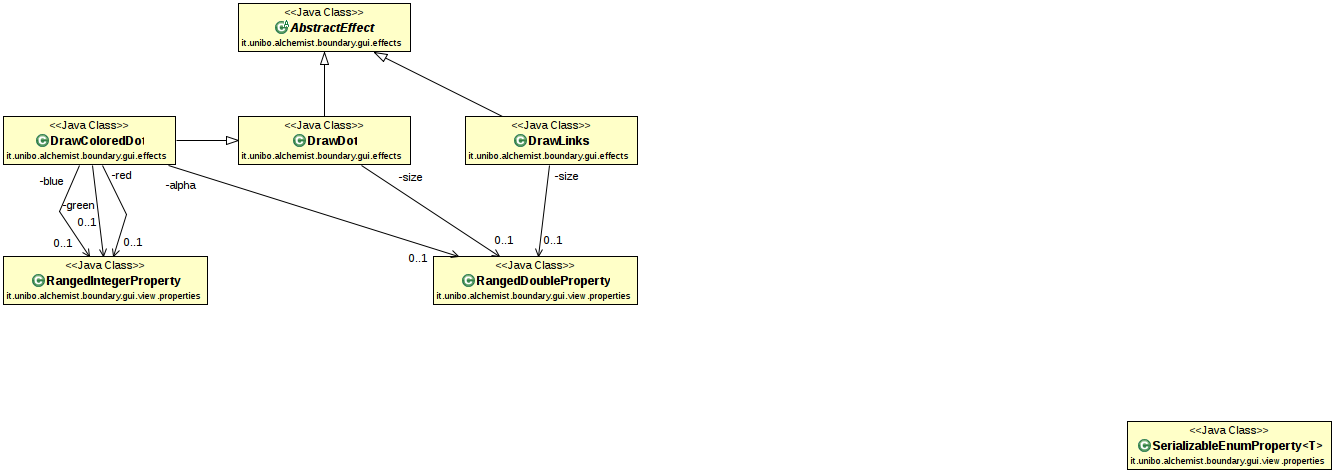
\includegraphics[scale=0.7]{img/EffectAndPropertiesUML}
                % \caption{Il diagramma UML delle classi mostra le relazioni tra gli effetti implementati e le proprietà custom utilizzate}
            % \end{figure}
